\documentclass[tikz,border=10pt]{standalone}
% No extra TikZ libraries needed.
\begin{document}
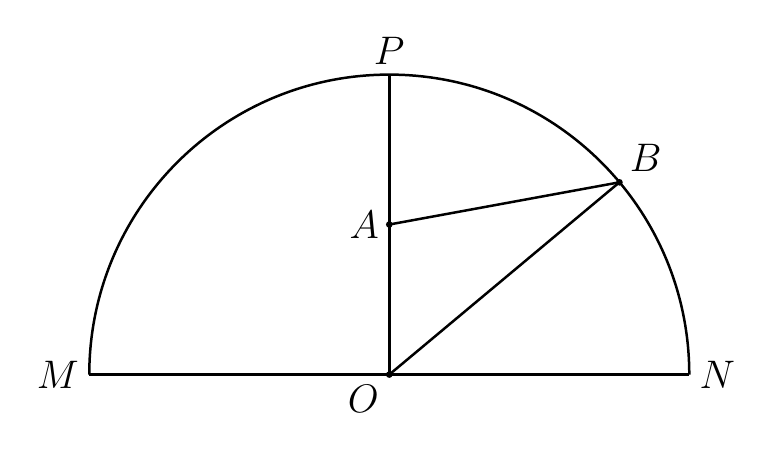
\begin{tikzpicture}[line width=0.9pt, line join=round]
  % Named coordinates (cm), scale s = 0.016064 cm/px, y flipped around O
  \coordinate (O) at (0,0);
  \coordinate (M) at (-3.81,0);
  \coordinate (N) at (3.81,0);
  \coordinate (P) at (0,3.81);
  \coordinate (A) at (0,1.906);
  \coordinate (B) at (2.923,2.442);

  % Semicircle (upper half) from M through P to N
  \draw (M) arc[start angle=180, end angle=0, radius=3.81];

  % Diameter MN
  \draw (M) -- (N);

  % Segment OP
  \draw (O) -- (P);

  % Segments AB and OB
  \draw (A) -- (B);
  \draw (O) -- (B);

  % Small filled dots at A and B
  \fill (A) circle (1.2pt);
  \fill (B) circle (1.2pt);

  % Labels: regular-weight math italic, same anchors
  \node[left]        at (M) {\fontsize{13.5}{16}\selectfont $M$};
  \node[right]       at (N) {\fontsize{13.5}{16}\selectfont $N$};
  \node[below left]  at (O) {\fontsize{13.5}{16}\selectfont $O$};
  \node[above]       at (P) {\fontsize{13.5}{16}\selectfont $P$};
  \node[left]        at (A) {\fontsize{13.5}{16}\selectfont $A$};
  \node[above right] at (B) {\fontsize{13.5}{16}\selectfont $B$};

  % Dot at O drawn last so it sits on top of the strokes
  \fill (O) circle (1.2pt);
\end{tikzpicture}
\end{document}